% Graphic for TeX using PGF
% Title: /home/jnicolaschc/GitHub/Teoría de Telecominicaciones I /ttl1_trabajo5/Documentos/Desarrollo/codigofuente/pgf/PlanPruebas.dia
% Creator: Dia v0.97+git
% CreationDate: Wed Sep 22 21:12:21 2021
% For: jnicolaschc
% \usepackage{tikz}
% The following commands are not supported in PSTricks at present
% We define them conditionally, so when they are implemented,
% this pgf file will use them.
\ifx\du\undefined
	\newlength{\du}
\fi
\setlength{\du}{15\unitlength}
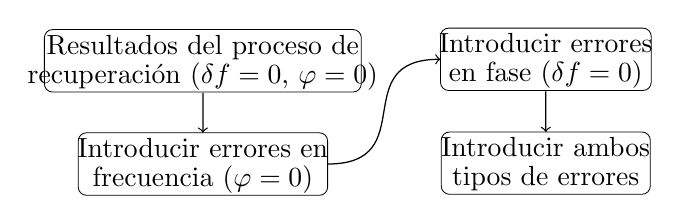
\begin{tikzpicture}[scale = 2]
	\pgftransformxscale{1.000000}
	\pgftransformyscale{-1.000000}
	\definecolor{dialinecolor}{rgb}{0.000000, 0.000000, 0.000000}
	\pgfsetstrokecolor{dialinecolor}
	\pgfsetstrokeopacity{1.000000}
	\definecolor{diafillcolor}{rgb}{1.000000, 1.000000, 1.000000}
	\pgfsetfillcolor{diafillcolor}
	\pgfsetfillopacity{1.000000}
	\pgfsetlinewidth{0.030000\du}
	\pgfsetdash{}{0pt}
	\pgfsetmiterjoin
	\pgfsetbuttcap
	{
		\definecolor{diafillcolor}{rgb}{0.000000, 0.000000, 0.000000}
		\pgfsetfillcolor{diafillcolor}
		\pgfsetfillopacity{1.000000}
		% was here!!!
		\pgfsetarrowsend{to}
		\definecolor{dialinecolor}{rgb}{0.000000, 0.000000, 0.000000}
		\pgfsetstrokecolor{dialinecolor}
		\pgfsetstrokeopacity{1.000000}
		\pgfpathmoveto{\pgfpoint{40.873221\du}{15.637061\du}}
		\pgfpathcurveto{\pgfpoint{42.012721\du}{15.637061\du}}{\pgfpoint{41.092668\du}{14.375616\du}}{\pgfpoint{42.232168\du}{14.375616\du}}
		\pgfusepath{stroke}
	}
	\pgfsetlinewidth{0.020000\du}
	\pgfsetdash{}{0pt}
	\pgfsetroundjoin
	\pgfsetbuttcap
	{\pgfsetcornersarced{\pgfpoint{0.200000\du}{0.200000\du}}\definecolor{diafillcolor}{rgb}{1.000000, 1.000000, 1.000000}
		\pgfsetfillcolor{diafillcolor}
		\pgfsetfillopacity{1.000000}
		\fill (42.241579\du,15.251430\du)--(42.241579\du,16.001678\du)--(44.759810\du,16.001678\du)--(44.759810\du,15.251430\du)--cycle;
	}{\pgfsetcornersarced{\pgfpoint{0.200000\du}{0.200000\du}}\definecolor{dialinecolor}{rgb}{0.000000, 0.000000, 0.000000}
		\pgfsetstrokecolor{dialinecolor}
		\pgfsetstrokeopacity{1.000000}
		\draw (42.241579\du,15.251430\du)--(42.241579\du,16.001678\du)--(44.759810\du,16.001678\du)--(44.759810\du,15.251430\du)--cycle;
	}% setfont left to latex
	\definecolor{dialinecolor}{rgb}{0.000000, 0.000000, 0.000000}
	\pgfsetstrokecolor{dialinecolor}
	\pgfsetstrokeopacity{1.000000}
	\definecolor{diafillcolor}{rgb}{0.000000, 0.000000, 0.000000}
	\pgfsetfillcolor{diafillcolor}
	\pgfsetfillopacity{1.000000}
	\node[anchor=base,inner sep=0pt, outer sep=0pt,color=dialinecolor] at (43.500694\du,15.547860\du){Introducir ambos};
	% setfont left to latex
	\definecolor{dialinecolor}{rgb}{0.000000, 0.000000, 0.000000}
	\pgfsetstrokecolor{dialinecolor}
	\pgfsetstrokeopacity{1.000000}
	\definecolor{diafillcolor}{rgb}{0.000000, 0.000000, 0.000000}
	\pgfsetfillcolor{diafillcolor}
	\pgfsetfillopacity{1.000000}
	\node[anchor=base,inner sep=0pt, outer sep=0pt,color=dialinecolor] at (43.500694\du,15.900638\du){tipos de errores};
	\pgfsetlinewidth{0.030000\du}
	\pgfsetdash{}{0pt}
	\pgfsetbuttcap
	{
		\definecolor{diafillcolor}{rgb}{0.000000, 0.000000, 0.000000}
		\pgfsetfillcolor{diafillcolor}
		\pgfsetfillopacity{1.000000}
		% was here!!!
		\pgfsetarrowsend{to}
		\definecolor{dialinecolor}{rgb}{0.000000, 0.000000, 0.000000}
		\pgfsetstrokecolor{dialinecolor}
		\pgfsetstrokeopacity{1.000000}
		\draw (43.501133\du,14.760495\du)--(43.500694\du,15.251430\du);
	}
	\pgfsetlinewidth{0.020000\du}
	\pgfsetdash{}{0pt}
	\pgfsetroundjoin
	\pgfsetbuttcap
	{\pgfsetcornersarced{\pgfpoint{0.200000\du}{0.200000\du}}\definecolor{diafillcolor}{rgb}{1.000000, 1.000000, 1.000000}
		\pgfsetfillcolor{diafillcolor}
		\pgfsetfillopacity{1.000000}
		\fill (37.869095\du,15.260524\du)--(37.869095\du,16.013598\du)--(40.873221\du,16.013598\du)--(40.873221\du,15.260524\du)--cycle;
	}{\pgfsetcornersarced{\pgfpoint{0.200000\du}{0.200000\du}}\definecolor{dialinecolor}{rgb}{0.000000, 0.000000, 0.000000}
		\pgfsetstrokecolor{dialinecolor}
		\pgfsetstrokeopacity{1.000000}
		\draw (37.869095\du,15.260524\du)--(37.869095\du,16.013598\du)--(40.873221\du,16.013598\du)--(40.873221\du,15.260524\du)--cycle;
	}% setfont left to latex
	\definecolor{dialinecolor}{rgb}{0.000000, 0.000000, 0.000000}
	\pgfsetstrokecolor{dialinecolor}
	\pgfsetstrokeopacity{1.000000}
	\definecolor{diafillcolor}{rgb}{0.000000, 0.000000, 0.000000}
	\pgfsetfillcolor{diafillcolor}
	\pgfsetfillopacity{1.000000}
	\node[anchor=base,inner sep=0pt, outer sep=0pt,color=dialinecolor] at (39.371158\du,15.554261\du){Introducir errores en};
	% setfont left to latex
	\definecolor{dialinecolor}{rgb}{0.000000, 0.000000, 0.000000}
	\pgfsetstrokecolor{dialinecolor}
	\pgfsetstrokeopacity{1.000000}
	\definecolor{diafillcolor}{rgb}{0.000000, 0.000000, 0.000000}
	\pgfsetfillcolor{diafillcolor}
	\pgfsetfillopacity{1.000000}
	\node[anchor=base,inner sep=0pt, outer sep=0pt,color=dialinecolor] at (39.371158\du,15.907039\du){frecuencia ($\varphi =0$)};
	\pgfsetlinewidth{0.020000\du}
	\pgfsetdash{}{0pt}
	\pgfsetroundjoin
	\pgfsetbuttcap
	{\pgfsetcornersarced{\pgfpoint{0.200000\du}{0.200000\du}}\definecolor{diafillcolor}{rgb}{1.000000, 1.000000, 1.000000}
		\pgfsetfillcolor{diafillcolor}
		\pgfsetfillopacity{1.000000}
		\fill (42.232168\du,13.999909\du)--(42.232168\du,14.751322\du)--(44.770786\du,14.751322\du)--(44.770786\du,13.999909\du)--cycle;
	}{\pgfsetcornersarced{\pgfpoint{0.200000\du}{0.200000\du}}\definecolor{dialinecolor}{rgb}{0.000000, 0.000000, 0.000000}
		\pgfsetstrokecolor{dialinecolor}
		\pgfsetstrokeopacity{1.000000}
		\draw (42.232168\du,13.999909\du)--(42.232168\du,14.751322\du)--(44.770786\du,14.751322\du)--(44.770786\du,13.999909\du)--cycle;
	}% setfont left to latex
	\definecolor{dialinecolor}{rgb}{0.000000, 0.000000, 0.000000}
	\pgfsetstrokecolor{dialinecolor}
	\pgfsetstrokeopacity{1.000000}
	\definecolor{diafillcolor}{rgb}{0.000000, 0.000000, 0.000000}
	\pgfsetfillcolor{diafillcolor}
	\pgfsetfillopacity{1.000000}
	\node[anchor=base,inner sep=0pt, outer sep=0pt,color=dialinecolor] at (43.501477\du,14.292816\du){Introducir errores};
	% setfont left to latex
	\definecolor{dialinecolor}{rgb}{0.000000, 0.000000, 0.000000}
	\pgfsetstrokecolor{dialinecolor}
	\pgfsetstrokeopacity{1.000000}
	\definecolor{diafillcolor}{rgb}{0.000000, 0.000000, 0.000000}
	\pgfsetfillcolor{diafillcolor}
	\pgfsetfillopacity{1.000000}
	\node[anchor=base,inner sep=0pt, outer sep=0pt,color=dialinecolor] at (43.501477\du,14.645593\du){en fase ($\delta f=0$)};
	\pgfsetlinewidth{0.020000\du}
	\pgfsetdash{}{0pt}
	\pgfsetroundjoin
	\pgfsetbuttcap
	{\pgfsetcornersarced{\pgfpoint{0.200000\du}{0.200000\du}}\definecolor{diafillcolor}{rgb}{1.000000, 1.000000, 1.000000}
		\pgfsetfillcolor{diafillcolor}
		\pgfsetfillopacity{1.000000}
		\fill (37.461308\du,14.017230\du)--(37.461308\du,14.770305\du)--(41.278696\du,14.770305\du)--(41.278696\du,14.017230\du)--cycle;
	}{\pgfsetcornersarced{\pgfpoint{0.200000\du}{0.200000\du}}\definecolor{dialinecolor}{rgb}{0.000000, 0.000000, 0.000000}
		\pgfsetstrokecolor{dialinecolor}
		\pgfsetstrokeopacity{1.000000}
		\draw (37.461308\du,14.017230\du)--(37.461308\du,14.770305\du)--(41.278696\du,14.770305\du)--(41.278696\du,14.017230\du)--cycle;
	}\pgfsetlinewidth{0.030000\du}
	\pgfsetdash{}{0pt}
	\pgfsetbuttcap
	{
		\definecolor{diafillcolor}{rgb}{0.000000, 0.000000, 0.000000}
		\pgfsetfillcolor{diafillcolor}
		\pgfsetfillopacity{1.000000}
		% was here!!!
		\pgfsetarrowsend{to}
		\definecolor{dialinecolor}{rgb}{0.000000, 0.000000, 0.000000}
		\pgfsetstrokecolor{dialinecolor}
		\pgfsetstrokeopacity{1.000000}
		\draw (39.370517\du,14.780168\du)--(39.371158\du,15.260524\du);
	}
	% setfont left to latex
	\definecolor{dialinecolor}{rgb}{0.000000, 0.000000, 0.000000}
	\pgfsetstrokecolor{dialinecolor}
	\pgfsetstrokeopacity{1.000000}
	\definecolor{diafillcolor}{rgb}{0.000000, 0.000000, 0.000000}
	\pgfsetfillcolor{diafillcolor}
	\pgfsetfillopacity{1.000000}
	\node[anchor=base,inner sep=0pt, outer sep=0pt,color=dialinecolor] at (39.370002\du,14.315074\du){Resultados del proceso de};
	% setfont left to latex
	\definecolor{dialinecolor}{rgb}{0.000000, 0.000000, 0.000000}
	\pgfsetstrokecolor{dialinecolor}
	\pgfsetstrokeopacity{1.000000}
	\definecolor{diafillcolor}{rgb}{0.000000, 0.000000, 0.000000}
	\pgfsetfillcolor{diafillcolor}
	\pgfsetfillopacity{1.000000}
	\node[anchor=base,inner sep=0pt, outer sep=0pt,color=dialinecolor] at (39.370002\du,14.667852\du){recuperación ($\delta f=0$, $\varphi =0$)};
\end{tikzpicture}
